\documentclass[letterpaper,12pt,oneside]{book}
\usepackage[top=1in, left=1.25in, right=1.25in, bottom=1in]{geometry}
\usepackage{bachelorstitlepageUNAM}

%%%%%%%%%%%%%%%%%%%%%%%%%%%%%
% Comparto una plantilla para la PORTADA que us\'e en mi t\'esis
% basada en el dise\~no gen\'erico que se usa en la Facultad de Ciencias
% Para usarlo \'unicamente aseg\'urate de tener la l\'inea
% \usepackage{bachelorstitlepageUNAM} y el archivo bachelorstitlepageUNAM.sty en el mismo directorio de trabajo.
% y los campos (sin signo %) :
%\author{Nombre del Alumno}
%\title{T\'itulo de la tesis}
%\faculty{Facultad}
%\degree{Grado que obtienes}
%\supervisor{ Tutor}
%\cityandyear{Ciudad y anio}
%\logouni{nombredelescudodelaunamsinespacios}
%\logofac{NombreDeLaImagenDelEscudodeTuFacultadSinEspacios}
% Para sugerencias y comentarios: DM en twitter.com/sglvgdor
% Subir\'e mas adelante la plantilla para maestr\'ia
%%%%%%%%%%%%%%%%%%%%%%%%%%%%%

\author{Pérez Romero Natalia Abigail}
\title{ ...}
\faculty{Facultad de Ciencias}
\degree{Licenciatura en Ciencias de la Computación}
\supervisor{Dr. José David Flores Peñaloza}
\cityandyear{Ciudad Universitaria, Cd. Mx., 2023}
\logouni{Escudo-UNAM}
\logofac{Escudo-FCIENCIAS}

\usepackage[T1]{fontenc}
\usepackage[utf8]{inputenc}
\usepackage[spanish,es-nodecimaldot,es-tabla]{babel}
\usepackage{graphicx}
\usepackage{tikz}
\usepackage{minted}
% use hyperref to make the table of contents clickable
\usepackage{hyperref}

\graphicspath{{"imagenes/"}}
\usepackage{setspace}
%\usepackage[round]{natbib}

\usepackage{lipsum}

\begin{document}
\frontmatter
\maketitle


\mainmatter

\chapter{title}

% Crear indice
\tableofcontents

\chapter{Introducción} %

% Introduccion, justificacion y objetivos
En la actualidad, y desde hace tiempo, las empresas al tener una presencia global con múltiples sucursales y empleados remotos requieren establecer conexiones seguras entre sus dispositivos. Para esto hay dos opciones: una línea de alquiler privada y dedicada o compartir una parte del ancho de banda con una línea existente, como Internet. La segunda opción es más económica y flexible, pero menos segura. De ahí surgen las redes privadas virtuales (VPN) que permiten establecer un túnel seguro dentro de una red pública tal como si estuvieran conectados en una red local. Adicionalmente, usuarios finales han encontrado en las VPN una forma de proteger su información y privacidad, además de acceder a contenido restringido geográficamente.

Diferentes protocolos de VPN han sido desarrollados para responder a estos requerimientos, cada uno con sus propias características y funcionalidades, entre ellos OpenVPN y IPsec. Sin embargo, estos protocolos presentan problemas de seguridad, complejidad y rendimiento. Por ejemplo, OpenVPN es un protocolo de VPN de código abierto que utiliza el protocolo SSL/TLS para cifrar el tráfico de red, pero es lento y complejo de configurar. Por otro lado, IPsec es un protocolo de VPN que utiliza el protocolo IKEv2 para establecer un túnel seguro, pero es difícil de configurar y no es compatible con todos los dispositivos.

En respuesta a estos problemas, se ha desarrollado un protocolo de VPN llamado WireGuard que es más simple, más rápido y más seguro que otros protocolos de VPN. WireGuard es más simple que otros protocolos de VPN porque utiliza un enfoque basado en claves públicas para establecer un túnel seguro, en lugar de utilizar certificados SSL/TLS como OpenVPN. WireGuard es más rápido que otros protocolos de VPN porque utiliza un enfoque basado en el kernel para cifrar y descifrar el tráfico de red, en lugar de utilizar un enfoque basado en el usuario como OpenVPN. WireGuard es más seguro que otros protocolos de VPN porque utiliza un enfoque basado en claves públicas para establecer un túnel seguro, en lugar de utilizar un enfoque basado en contraseñas como IPsec.

Si bien WireGuard es un protocolo de VPN simple, la mayor de sus desventajas es la configuración de los pares dentro de la red. Por ejemplo, si se desea configurar una red privada virtual con 10 pares, se debe configurar manualmente cada par con la dirección IP y la clave pública de cada par. Esto puede ser un proceso tedioso y propenso a errores, especialmente si se desea configurar una red privada virtual con un gran número de pares.

Una solución para esta dificultad es propuesa por Tailscale, el cual es un servicio VPN que hace que sus dispositivos y aplicaciones sean accesibles en cualquier parte del mundo, de forma segura y sin esfuerzo. Este software actúa en combinación con el kernel para establecer una comunicación VPN peer-to-peer o retransmitida con otros clientes utilizando el protocolo WireGuard. Tailscale puede abrir una conexión directa con el peer utilizando técnicas de NAT traversal como STUN o solicitar el reenvío de puertos a través de UPnP IGD, NAT-PMP o PCP. [7] Si el software no consigue establecer una comunicación directa, recurre al protocolo DERP (Designated Encrypted Relay for Packets) proporcionados por la empresa. [6] Las direcciones IPv4 asignadas a los clientes se encuentran en el espacio reservado NAT de nivel operador. Esto se eligió para evitar interferencias con las redes existentes[9] ya que el enrutamiento de tráfico a redes detrás del cliente es posible.

Tailscale es una gran solución para la configuración de pares en WireGuard, pero no es una solución de código abierto. Al ofrecer más funcionalidades que las necesarias para la configuración de pares en WireGuard, Tailscale puede ser una solución costosa para empresas pequeñas o individuos que solo requieren configurar pares en WireGuard. Además, Tailscale no permite a los usuarios tener control total sobre la configuración de pares en WireGuard, ya que la configuración de pares en WireGuard se realiza a través de la interfaz de usuario de Tailscale y no a través de la línea de comandos. Y finalmente, Tailscale aumenta la superficie de ataque de la red privada virtual, ya que no solicita la autenticación al usar un servicio crítico como SSH entre los pares.

Existe una alternativa de código abierto del servidor de control de Tailscale llamado Headscale. El objetivo de Headscale es proporcionar a un servidor de código abierto que puedan utilizar para proyectos y laboratorios. Implementa un alcance estrecho, una sola Tailnet, adecuada para un uso personal o una pequeña organización de código abierto. [10]


Aunque Headscale sea una opción open-source no cuenta con un cliente en el dispositivo final y únicamente permite crear un red privada.

Por lo que en este trabajo se propone el desarrollo de un prototipo open-source de un sistema de control de configuración de pares minimalista usando el protocolo WireGuard, inspirado en Tailscale, el cual se adherirá a los principios de UNIX.

Este prototipo de sistema permitirá automatizar la configuración de pares, mediante:
\begin{itemize}
    \item \textbf{Cliente}: Programa que se ejecutará en el dispositivo final, el cual consiste de:
    \begin{itemize}
        \item \textit{Cliente daemon}: Un servidor XML-RPC que actuará como daemon guardando, actualizando y manteniendo la configuración actual de los pares y el cliente.
        \item \textit{Interfaz de cliente}: Un programa que actuará como interfaz recibiendo instrucciones por CLI e interactuando con el cliente daemon.
    \end{itemize}
    \item \textbf{Servidor Orquestador (LinkGuard)}: Un servidor XML-RPC que se encargará de orquestar y automatizar la configuración de los pares dentro de las redes privadas.
\end{itemize}


Se espera que este prototipo automatice la configuración de los pares en una VPN WireGuard, permitiendo que el servidor orquestador actúe como directorio conociendo la dirección IP del endpoint, puertos, llaves públicas, lista de IPs permitidas por cada par en cada red privada. También permitirá la comunicación entre dispositivos finales que no pueden comunicarse directamente, ya que actuará como intermediario en la comunicación.

Se espera que este prototipo reduzca la superficie de ataque de la red privada virtual al no realizar más funcionalidad que la orquestación de los pares en WireGuard. 


Para evaluar el prototipo se propondrán tres escenarios con dos dispositivos finales:
\begin{itemize}
    \item \textbf{Todos los dispositivos finales son alcanzables}: Es decir, tanto el orquestador como los dispositivos finales pueden comunicarse entre sí porque están en la misma red o cuentan con IPs públicas. No existen restricciones como firewalls o NATs.
    
    \item \textbf{Uno de los dispositivos es alcanzable}: En este escenario, el orquestador y los dispositivos final pueden comunicarse entre sí, pero uno dispositivo final no tiene una IP pública o está detrás de un NAT. De forma que el orquestador actuará como intermediario en la comunicación.
    
    \item \textbf{Solo el Orquestador es alcanzable}: Los dispositivos finales no pueden comunicarse entre sí directamente, pero pueden comunicarse con el orquestador, que actuará como intermediario en la comunicación.
\end{itemize}


% Definiciones
%
\section{VPN} %
Las VPN (Virtual Private Netwo  k) son redes privadas virtuales que permiten a los usuarios conectarse a una red privada a través de una red pública, como Internet. Las VPN se utilizan para proteger la privacidad y la seguridad de la información transmitida a través de la red.



\section{WireGuard}


\section{Tailscale}



\section{NAT}


\section{Firewall}

\chapter{Desarrollo}
%2. Desarrollo \> \dotfill  \\

%\hspace{0.5cm}2.0 Objetivos del programa \> \dotfill  \\
%\hspace{0.5cm}2.1 Funcionalidad del orquestrador \> \dotfill  \\
%\hspace{0.5cm}2.2 Descripcion del orquestrador \> \dotfill  \\
%\hspace{0.5cm}2.3 Componentes del orquestrador \> \dotfill  \\
%\hspace{0.5cm}2.4 Flujo del programa \> \dotfill  \\
%\hspace{0.5cm}2.5 Casos de uso \> \dotfill  \\


El objetivo principal es desarrollar un prototipo open-source de un sistema de control de configuración de pares minimalista usando el protocolo WireGuard, inspirado en Tailscale y adherido a los principios de UNIX de modularidad, claridad, composición, separación, simplicidad, transparencia, solidez, representación, menor sorpresa, silencio y reparación. Este sistema tiene la finalidad de automatizar la configuración y sincronización de pares en una VPN WireGuard.

Permitirá a los usuarios automatizar la configuración de los pares de una VPN WireGuard mediante un servidor orquestador y un cliente que se ejecutará en el dispositivo final. De forma que el cliente en el dispositivo final recibirá una vez la configuración por CLI de los pares y la mantendrá actualizada gracias a que enviará esta información al servidor orquestador que actuará como directorio conociendo la dirección IP del endpoint, puertos, llaves públicas, lista de IPs permitidas por cada par en cada red privada. Además, el servidor orquestador permitirá la comunicación entre dispositivos finales que no pueden comunicarse directamente, ya que actuará como intermediario en la comunicación.

Finalmente en este trabajo se validara la funcionalidad y robustez del prototipo mediante pruebas en diferentes escenarios, evaluando su impacto en la simplificación de la configuración y gestión de redes VPN WireGuard.

\section{Casos de uso}
\subsection{Identificación del usuario}

En esta primera version no nos preocuparemos de que la información del usuario se transmita de forma segura, por lo que el usuario deberá ingresar su nombre y contraseña en texto plano. Y se enviará al servidor para su verificación.

\begin{figure}
    \centering
    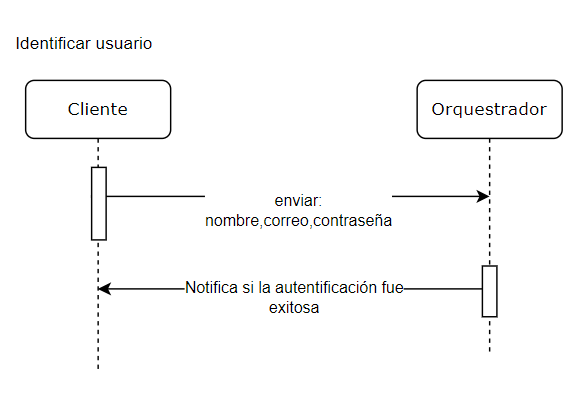
\includegraphics[width=\textwidth]{login-user.png}
    \caption{Pantalla de inicio de sesión}
\end{figure}

\subsubsection{Registro de usuario}

De igual forma el registro de usuario se hará en texto plano, y se enviará al servidor para su verificación.

\begin{figure}
    \centering
    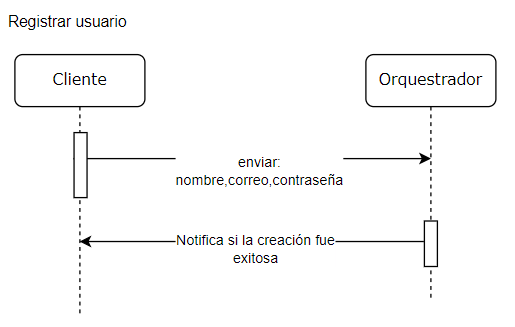
\includegraphics[width=\textwidth]{register-user.png}
    \caption{Pantalla de registro de usuario}
\end{figure}

\subsection{Registro de usuario}

\lipsum[1-2]
\newpage
\subsection{Conexión de dispositivos finales}

Tendremos dos casos en cuando se quieran conectar dos o más dispositivos finales, el primero es cuando es posible que se comuniquen entre si por que tienen direcciones IP ruteables.
El segundo caso es cuando los dispositivos finales no pueden comunicarse entre si por que no tienen direcciones IP ruteables, en este caso el orquestrador deberá ofrecer un mecanismo para que los dispositivos finales puedan conectarse entre sí mediante un relay.
\begin{figure}[h!]
    \centering
    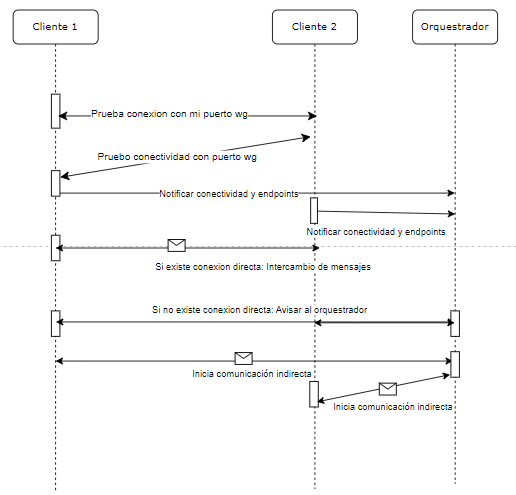
\includegraphics[width=\textwidth]{alcanzabilidad.png}
    \caption{Diagrama de caso de uso: conexión de dispositivos finales}
\end{figure}

\subsubsection{Conexión de dispositivos finales con direcciones IP ruteables. Directa}

En este caso el uno de los clientes se comunica directamente con el otro cliente, el orquestrador deberá enviar un mensaje de confirmación al cliente que solicita la conexión. 
Para esto el cliente A enviara mediante ping al cliente B a la dirección IP y puerto que el orquestrador le proporcionó para la interfaz Wireguard.

Si se obtiene una respuesta entonces consideramos que la conexión fue exitosa (los dispositivos son alcanzables). 
\begin{figure}[h!]
    \centering
    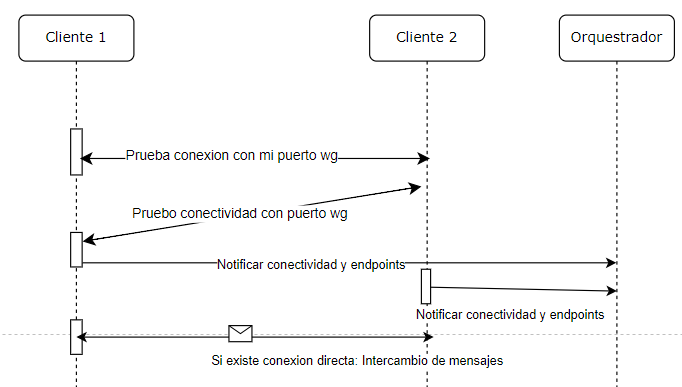
\includegraphics[width=\textwidth]{conexion-directa.png}
    \caption{Diagrama de caso de uso: conexión de dispositivos finales con direcciones IP ruteables. Directa}
\end{figure}


\subsubsection{Conexión de dispositivos finales con direcciones IP no ruteables. Relay}

En este caso el orquestrador deberá ofrecer un mecanismo para que los dispositivos finales puedan conectarse entre sí mediante un relay. 
El cliente A se comunica con el orquestrador para solicitar la conexión con el cliente B, el orquestrador deberá enviar un mensaje de confirmación al cliente A con la dirección IP y puerto del orquestrador, el cliente A deberá enviar un mensaje al orquestrador para que este se comunique con el cliente B. 

\begin{figure}[h!]
    \centering
    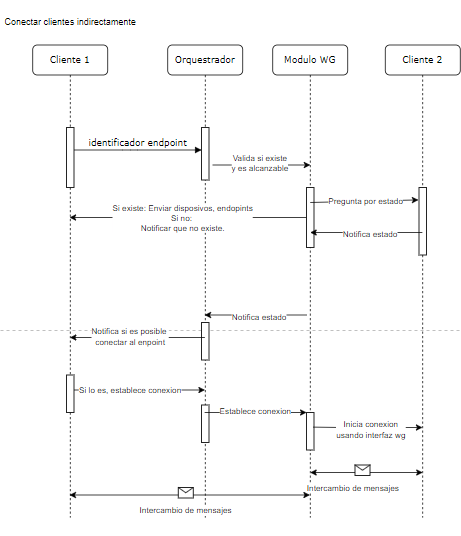
\includegraphics[width=\textwidth]{conecta-clientes-indirectamente.png}
    \caption{Diagrama de caso de uso: conexión de dispositivos finales con direcciones IP no ruteables. Relay}
\end{figure}

\newpage
\section{Diagrama de clases}
Para el orquestrador tendremos las siguientes clases:
\begin{figure}[h!]
    \centering
    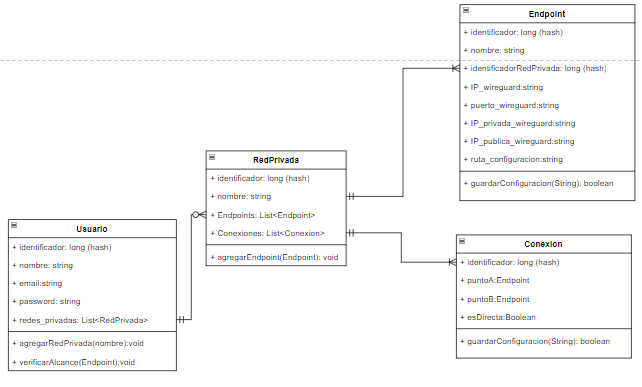
\includegraphics[width=\textwidth]{diagrama-clases.png}
    \caption{Diagrama de clases}
\end{figure}

Bajo la idea de que el orquestrador es el encargado de orquestar la conexión entre los dispositivos finales dentro de una red privada de un cliente, tendremos las siguientes clases:
\begin{itemize}
    \item \textbf{Cliente}: Clase que representa a un cliente que se conecta a la red privada de otro cliente.
    \item \textbf{Endpoiny}: Clase que representa a un dispositivo final que se conecta a la red privada de un cliente.
    \item \textbf{Conexión}: Clase que representa una conexión entre dos dispositivos finales. La idea de esta clase es que el orquestrador sepa que dispositivos finales están conectados entre si y para cuales es necesario relay.
\end{itemize}
%\lipsum[1-2]

\chapter{Resultados}  %

\chapter{Conclusiones}  %

\bibliographystyle{humannat}
%\bibliography{references}

\backmatter@sglvgdor

% Referencias
%https://www.overleaf.com/learn/latex/Bibliography_management_with_bibtex

\begin{thebibliography}{9}
\bibitem{computerNetworking}
  Kurose, J. F., \& Ross, K. W. (2017).
  \emph{Computer networking: a top-down approach},
  Pearson,
  7th edition.

\bibitem{wireguard}
    WireGuard,
    \emph{WireGuard: fast, modern, secure VPN tunnel},
    \url{https://www.wireguard.com/},
    2021.

\bibitem{linuxNetworkingGuide}
    Linux Documentation Project,
    \emph{Linux Advanced Routing \& Traffic Control HOWTO},
    \url{https://tldp.org/HOWTO/Adv-Routing-HOWTO/index.html},
    2021.

\bibitem{networkAdministartionGuide}
    Bautts, M., \& Dawson, M. (2000).
    \emph{Linux Network Administrator's Guide},
    O'Reilly Media,
    3rd edition.

% https://tldp.org/HOWTO/IP-Masquerade-HOWTO/kernel-2.4.x-requirements.html

\bibitem{ipMasquerade}
    Bautts, M., \& Dawson, M. (2000).
    \emph{Linux IP Masquerade HOWTO},
    \url{https://tldp.org/HOWTO/IP-Masquerade-HOWTO/index.html},
    2021.

\end{thebibliography}

\end{document}